\documentclass{report}
\usepackage{hyperref}
\usepackage[ngerman]{babel}
\usepackage{amsmath}
\usepackage{amsfonts}
\usepackage{amsthm}
\usepackage{tcolorbox}
\usepackage[a4paper, total={7in, 9in}]{geometry}
\usepackage[font={scriptsize,it}]{caption}
\usepackage{scrextend}
\usepackage{graphicx}
\usepackage{caption}
\usepackage{subcaption}
\usepackage[utf8]{inputenc}
\usepackage[T1]{fontenc}
\DeclareUnicodeCharacter{2212}{-}
\usepackage{verbatim}
\usepackage{tikz}

\tikzset{
  treenode/.style = {shape=rectangle, rounded corners,
                     draw, align=center,
                     top color=white, bottom color=blue!20},
  root/.style     = {treenode, font=\Large, bottom color=red!30},
  env/.style      = {treenode, font=\ttfamily\normalsize},
  dummy/.style    = {circle,draw}
}

\tikzstyle{level 1}=[level distance=3.5cm, sibling distance=3.5cm]
\tikzstyle{level 2}=[level distance=3.5cm, sibling distance=2cm]

% floating figure for column
\newenvironment{Figure}
	{\par\medskip\noindent\minipage{\linewidth}}
	{\endminipage\par\medskip}

\begin{document}

\begin{titlepage}
   \vspace*{\stretch{1.0}}
   \begin{center}
      \Large\textbf{eHealth Lab04 - HS20}\\
      \large\textit{Results from Ristovski Vele - ristovel and Pascal Brunner - brunnpa7}
   \end{center}
   \vspace*{\stretch{2.0}}
\end{titlepage}

% Beispiel Bild
%\begin{Figure}
%   \centering
%    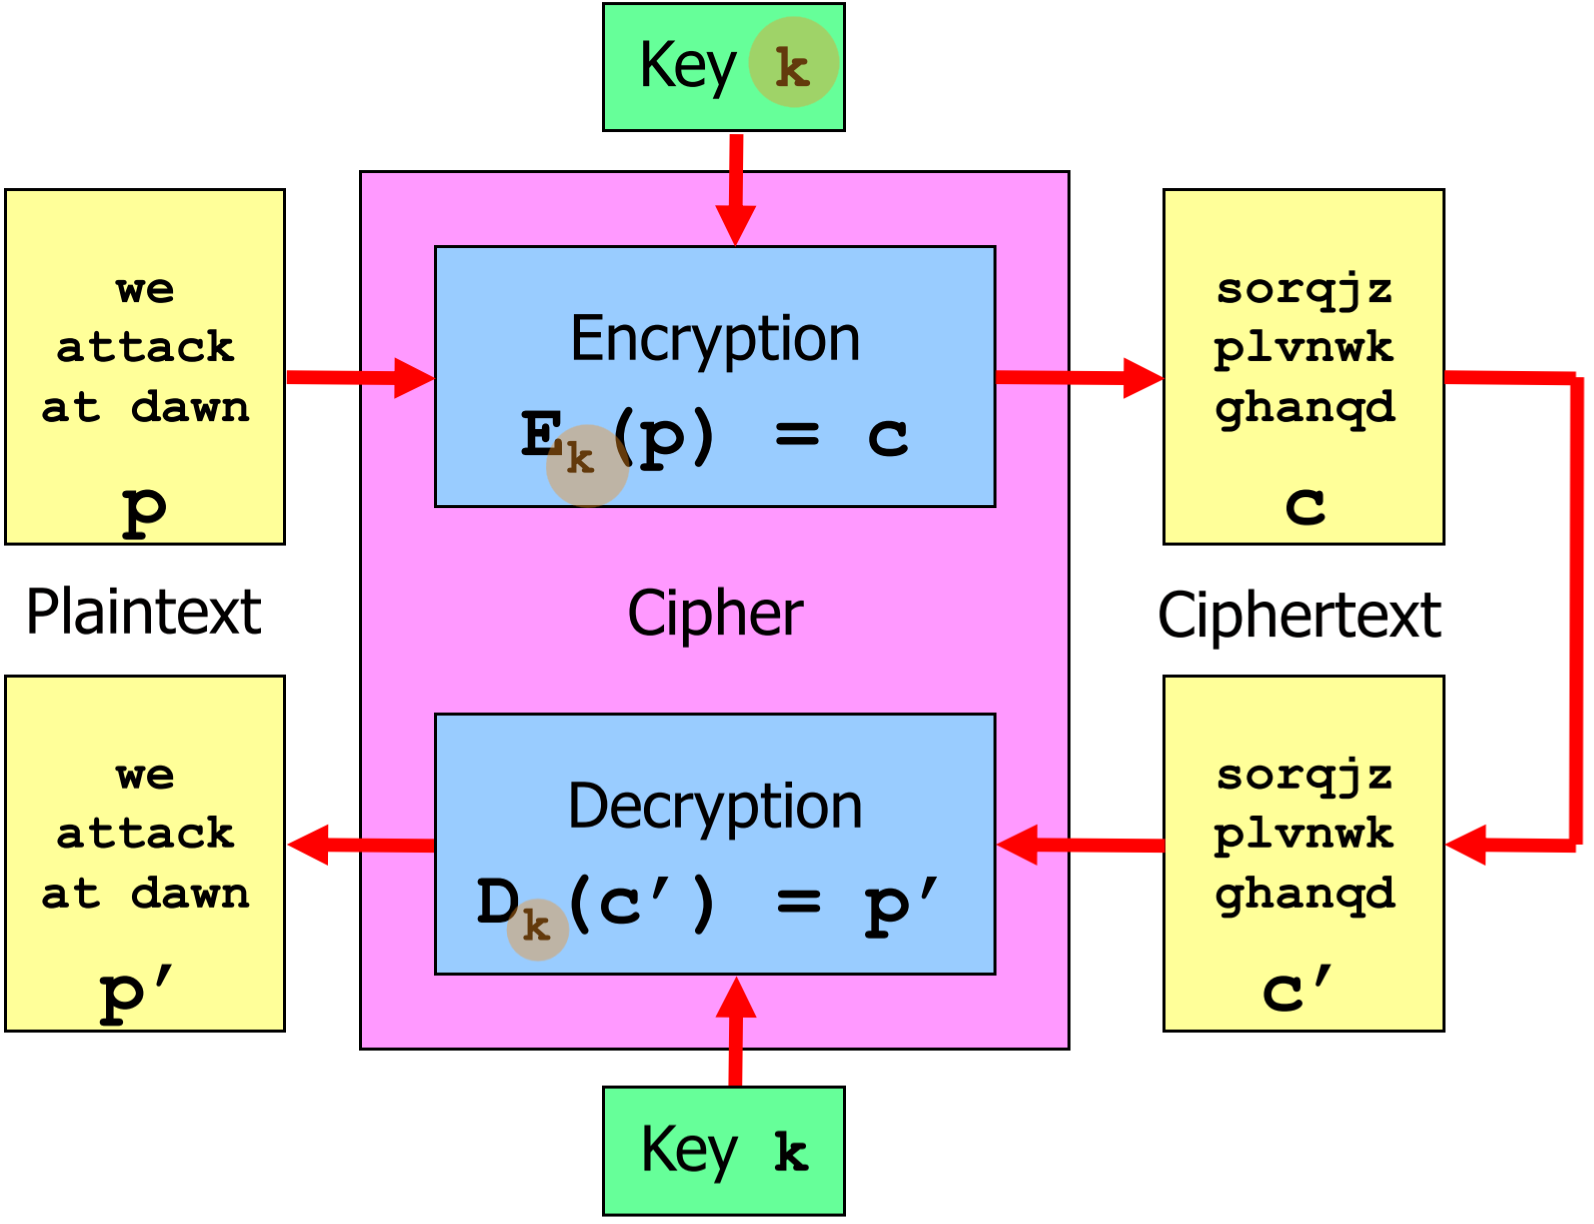
\includegraphics[width=300px]{img/BasicTerminologySecKeyCrypto.png}
%        \captionof{figure}{Basic Terminology basierend auf Secret Key Cryptography}
%        \label{fig:Basic Terminology}
%    \end{Figure}

\section*{Lab 04}

\textbf{Task 1}: Downloaded all papers

\textbf{Task 2.1: What means the oid 2.16.756.5.30.1.127.3.10.3?}\\
$\rightarrow$ EPR Sectorial Personal Identification Number (Patient Identification Number)
\begin{Figure}
   \centering
    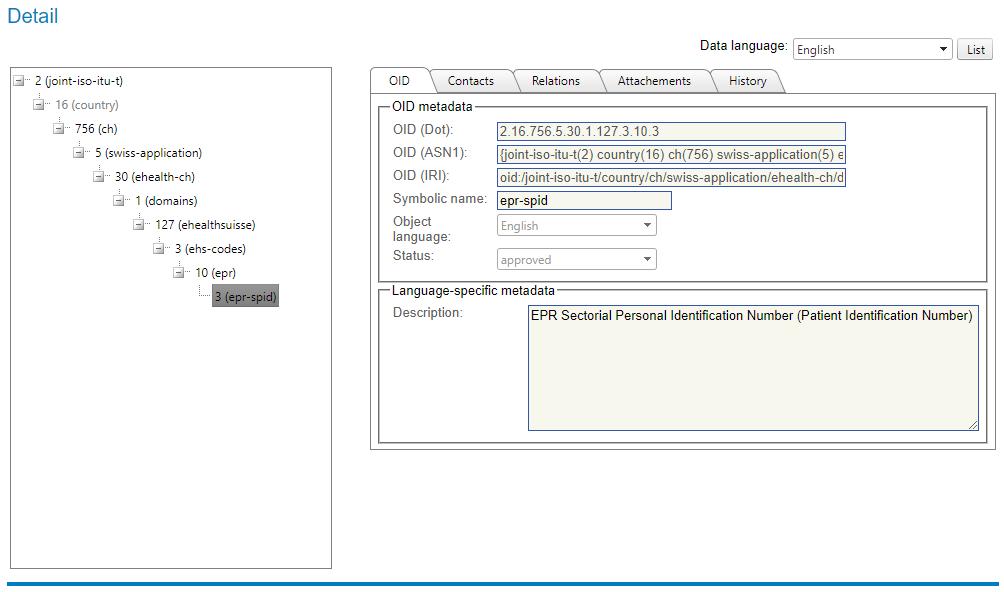
\includegraphics[width=300px]{img/OID.png}
        \captionof{figure}{Result by searching OID}
        \label{fig:Result by searching OID}
    \end{Figure}

\textbf{Task 2.2: Can you infer from 2.1 what is the meaning of the extension based on the root oid?}\\
$\rightarrow$ It is an unique ID to a person or company, which is issued by the root-id in our case \textit{eHealth-Suisse Koordinationsorgan Bund - Kantone}

\textbf{Task 2.3: Read up on the profile and the transaction in Volume 1 (2.2.23 Patient Identifier
Cross-referencing HL7 V3 (PIXV3)) and Volume 2b (3.45 PIXV3 Query [ITI-45]).}

\begin{Figure}
   \centering
    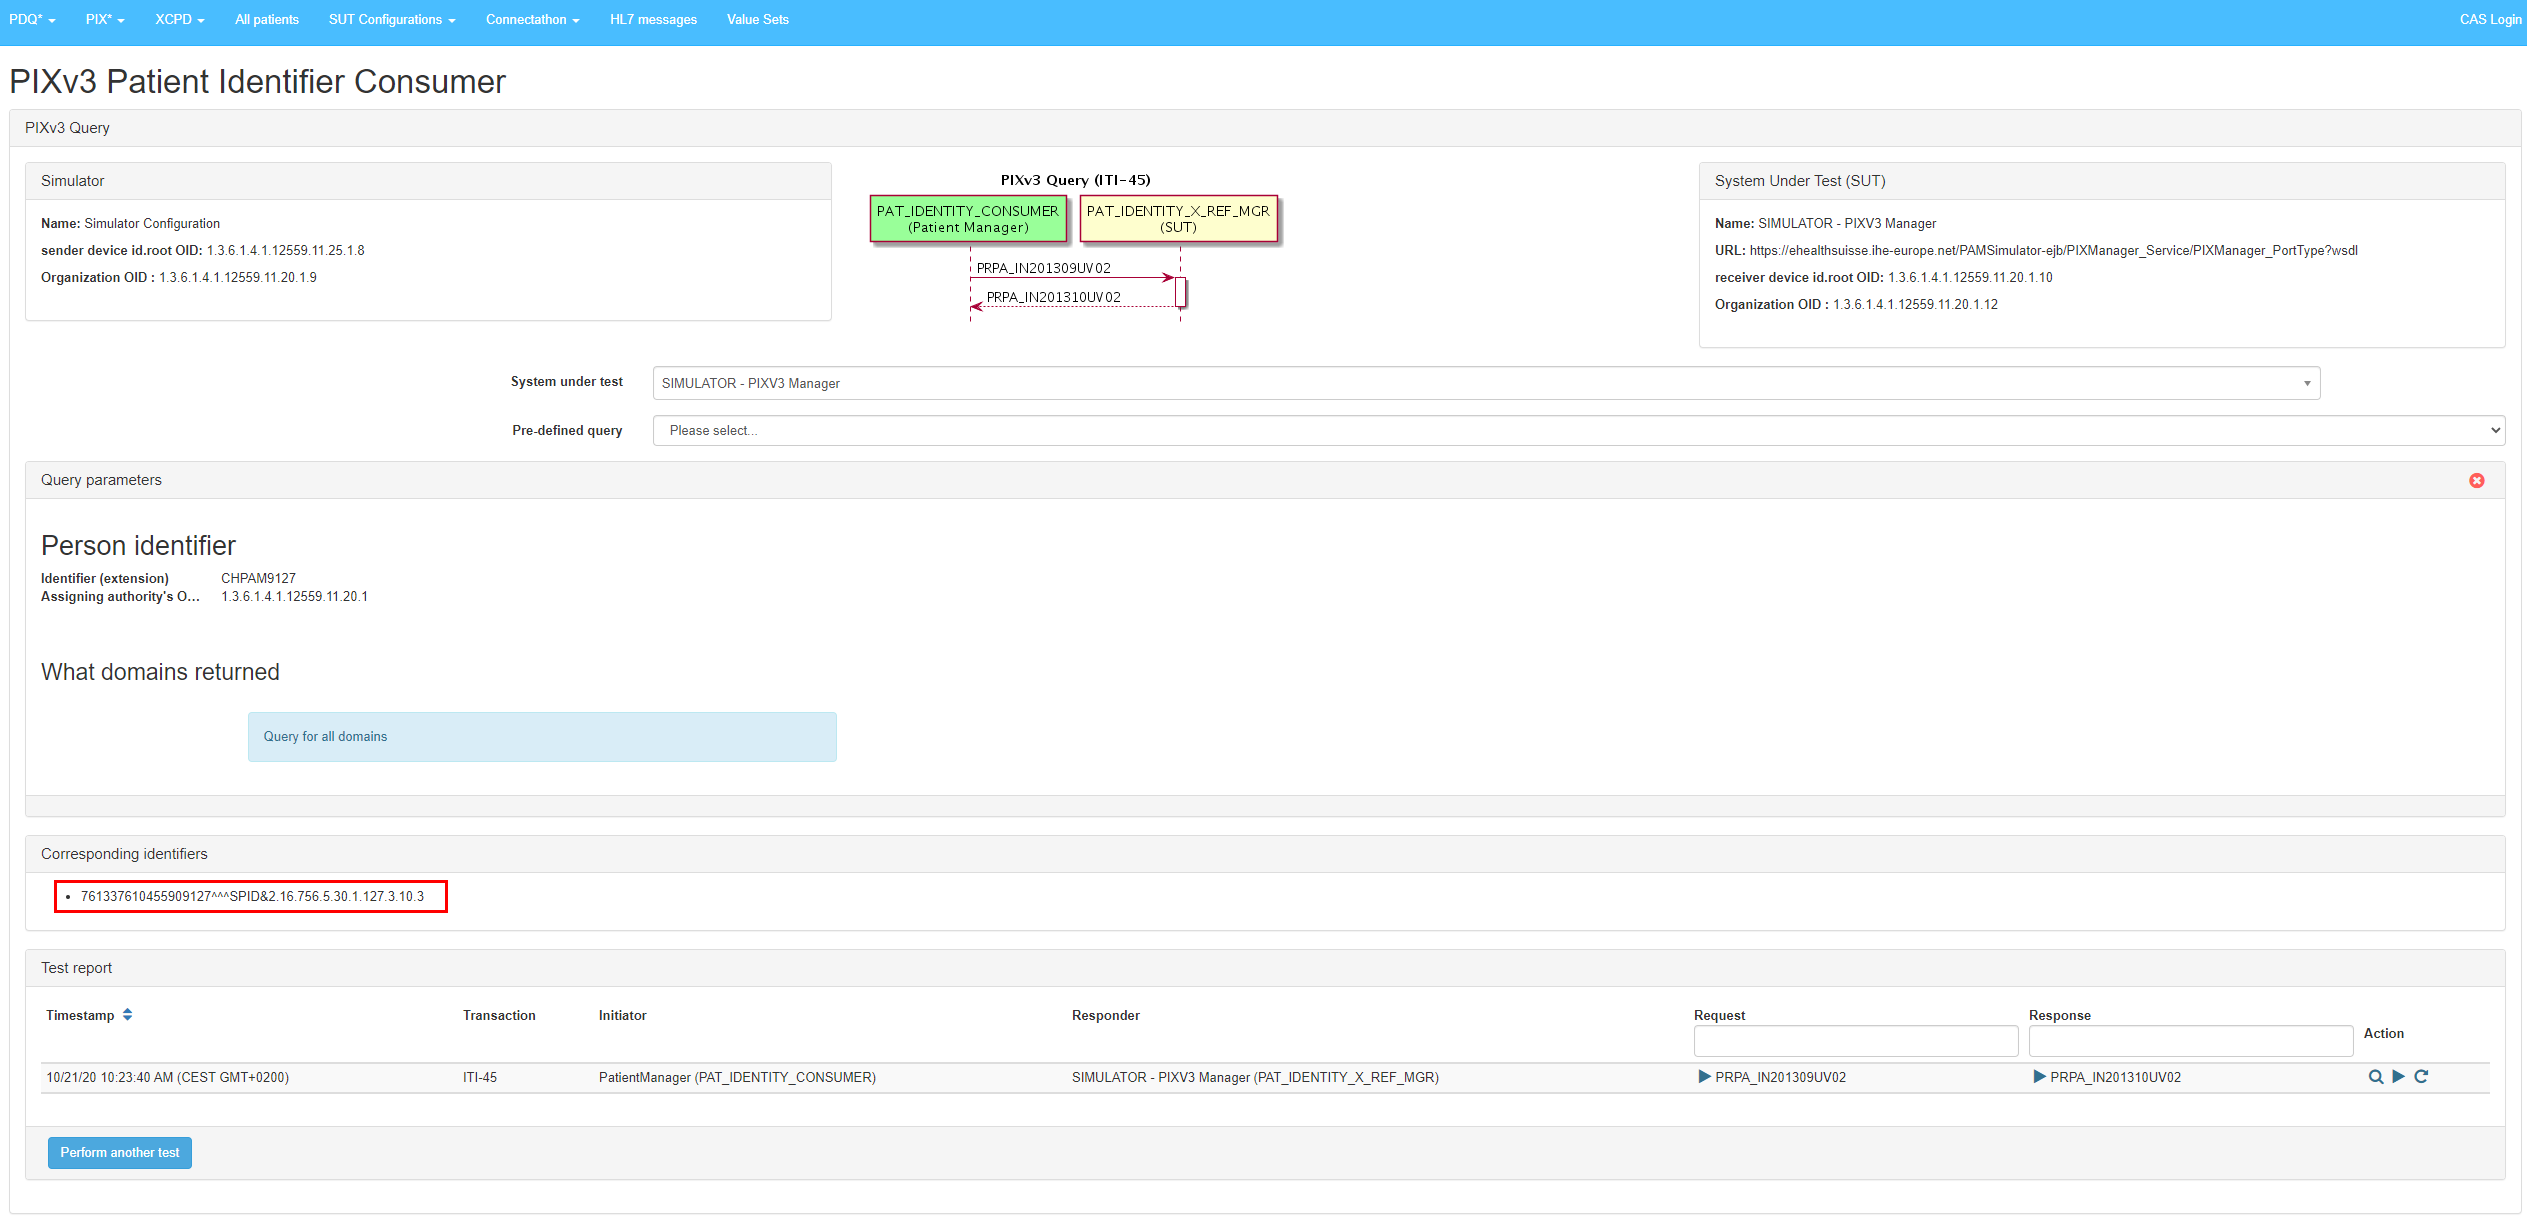
\includegraphics[width=300px]{img/Task23.png}
        \captionof{figure}{Result Task 2.3}
        \label{fig:Result Task 2.3}
    \end{Figure}

\textbf{Task 2.4: Perform the query directly in RESTClient / VS Code from}
\begin{enumerate}
   \item Get the address where you need to POST the XML with SOAP envelope from the following wsdl file description wsdl:service/wsdl:port/soap12:address location \url{https://ehealthsuisse.ihe-europe.net/PAMSimulator-ejb/PIXManager_Service/PIXManager_PortType?wsdl}
   \item Make a new POST Request with the XML with SOAP Envelope for and fill out the request like in Task 2.4.
   \item Perform the request till you get a response. Change the local identifier to CHPAM9810 and note the EPR-SPID as a result.
\end{enumerate}

$\rightarrow$ See Code-Snippet in zip-file\\

\textbf{Task 3: Provide and register a document for a patient}

\textbf{Task 3.1: Read up on the profile and the transaction in Volume 1 (10 Cross-Enterprise Document Sharing (XDS.b)) and Volume 2b (3.41 Provide and Register Document Set-b [ITI-41]).}\\
done

\textbf{Task 3.2 Prepare a PDF File to upload for the patient.}\\
We created a PDF-File with a radiology-picture for our imaginary patient \textit{Max Mustermann}

\textbf{Task 3.3 Use the XDStarClient as a Client to construct the ITI-41 Provide and Register Request for your PDF document (Menu SIMU-Initiators, IHE ITI, XDS.b, ITI-41).}
\begin{Figure}
   \centering
    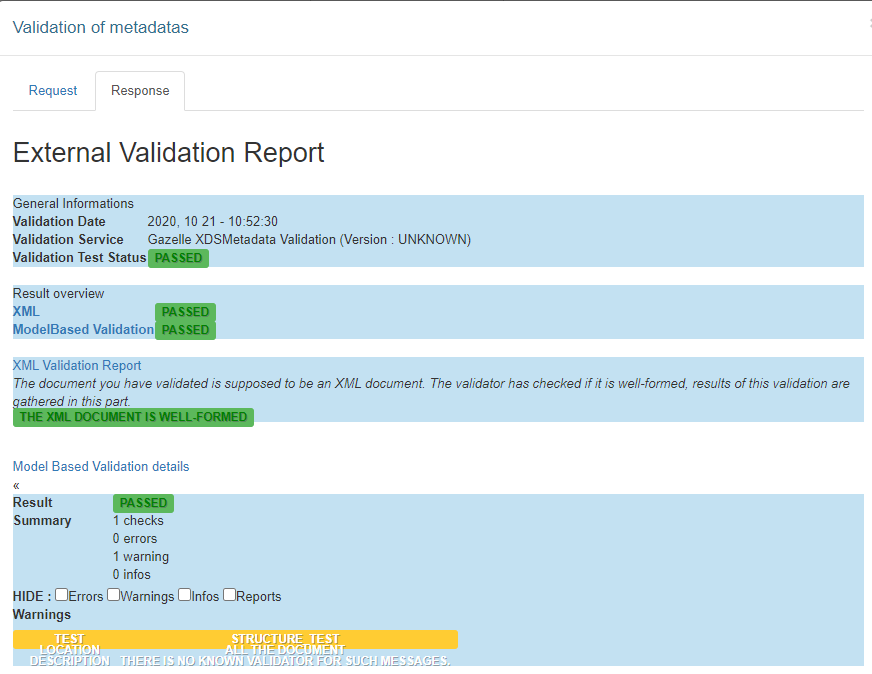
\includegraphics[width=300px]{img/Task33.png}
        \captionof{figure}{Result Task 3.3}
        \label{fig:Result Task 3.3}
    \end{Figure}
$\rightarrow$ See Code-Snippet in zip-file\\

\end{document}